\subsection{Dynamics results}
\label{subsec:molecular_dynamics_results}

First we look into relaxation of the order parameter to the equilibrium values. For that we perform Langevin Dynamics simulation for a set of simulation parameters as described in \ref{subsec:simulation_details}.

We start by looking into system evolution on a short time scale. For that we analyse time dependence of the order parameter~\eqref{eq:nematic_order_parameter} starting from different initial configurations outlined in previous section. The results for different densities are presented on the Figure~\ref{fig:short_time_order_parameter_different_density}. The squares stands for random initial configuration, the circles for co-aligned and triangles for counter-aligned initial configuration. Solid lines are linear approximation to the obtained results on the range $t \in (10, 100]$. 

Done in the $log-log$ coordinates, the Figure~\ref{fig:short_time_order_parameter_different_density} clearly shows power-law decay of order parameter to the equilibrium values for low density $\rho \le 0.5$ independent of the initial configuration.

\begin{figure}[h]
\centering
\begin{subfigure}[t]{0.32\textwidth}
	\centering
	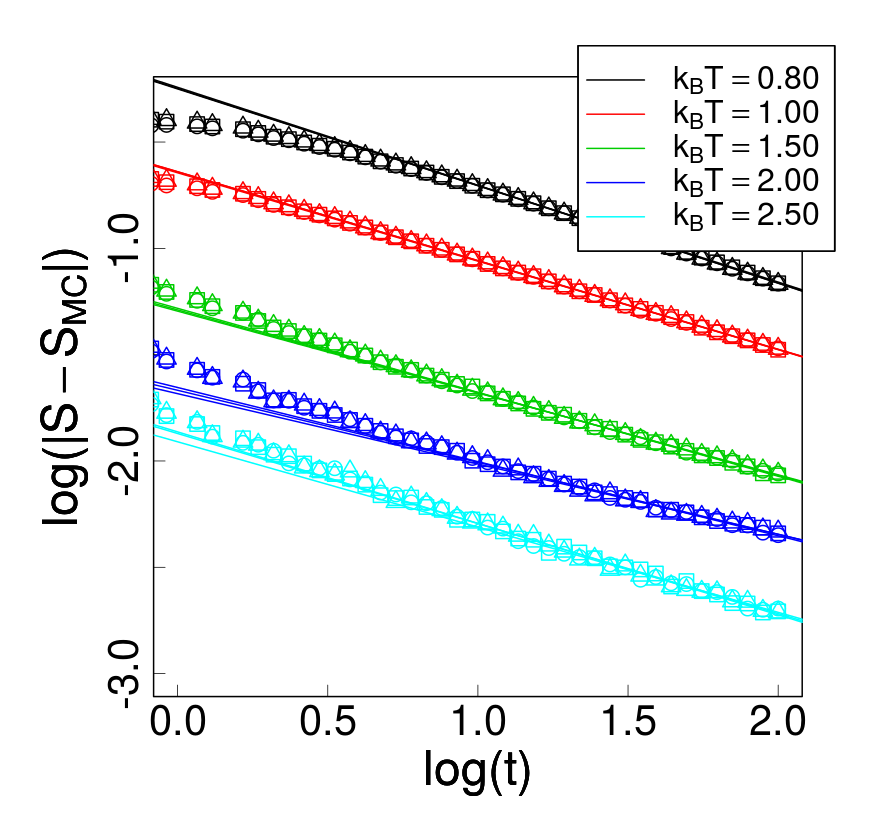
\includegraphics[width=\textwidth]{Images/relax_25.png}
	\captionsetup{justification=centering, width=0.9\columnwidth}
	\caption{$\rho = 0.25$}
\end{subfigure}
\begin{subfigure}[t]{0.32\textwidth}
	\centering
	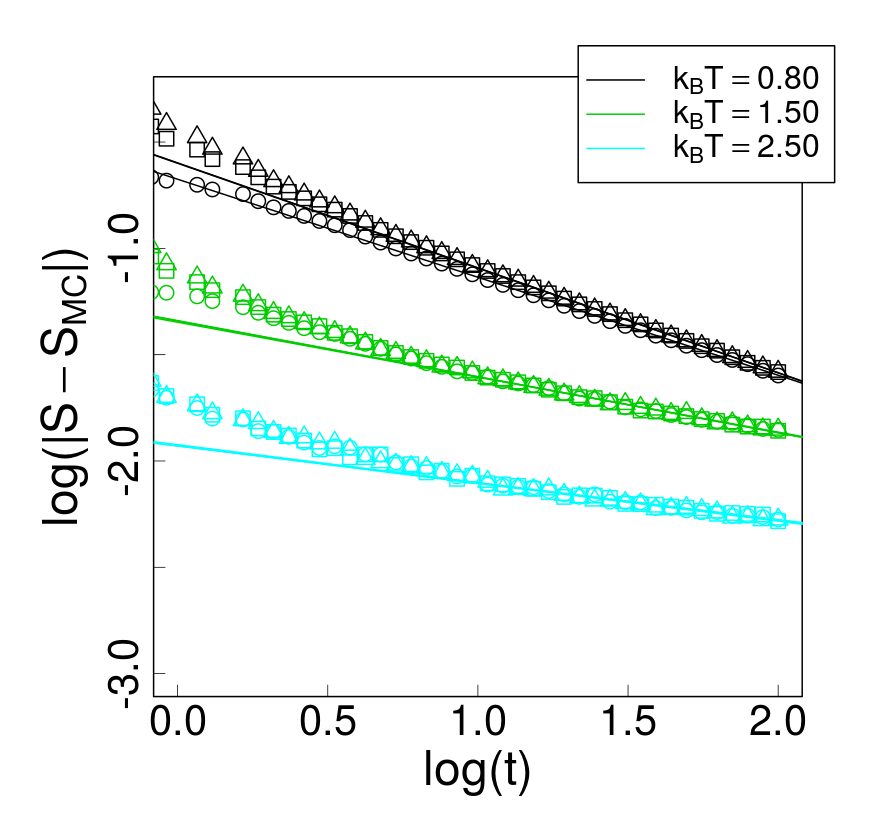
\includegraphics[width=\textwidth]{Images/relax_50.png}
	\captionsetup{justification=centering, width=0.9\columnwidth}
	\caption{$\rho = 0.5$}
\end{subfigure}
\begin{subfigure}[t]{0.32\textwidth}
	\centering
	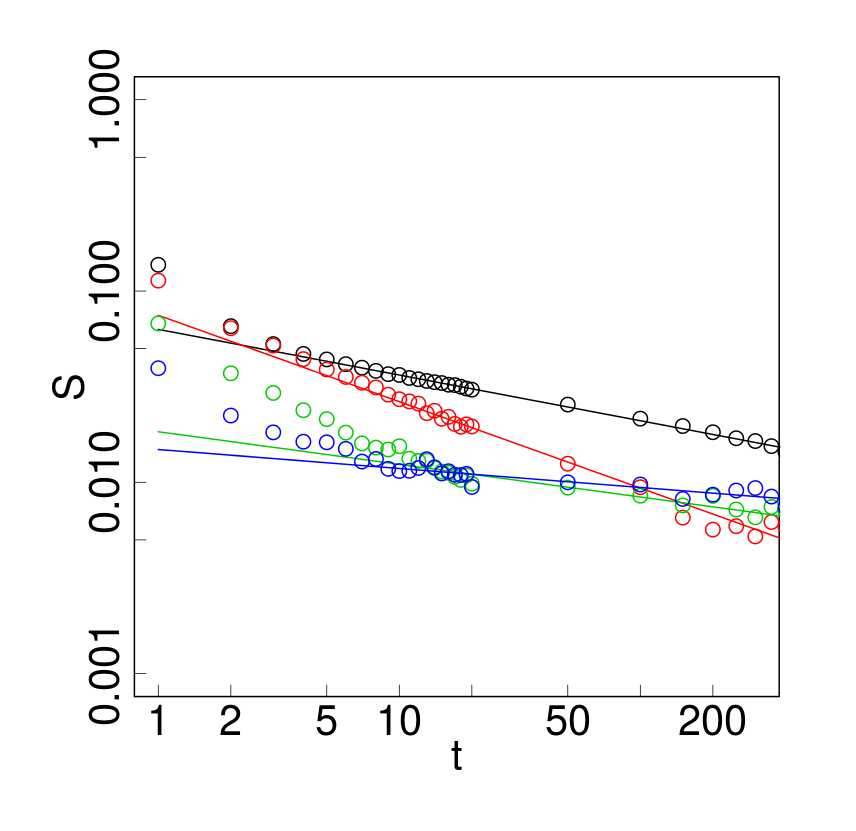
\includegraphics[width=\textwidth]{Images/relax_75.png}
	\captionsetup{justification=centering, width=0.9\columnwidth}
	\caption{$\rho = 0.75$}
\end{subfigure}
\captionsetup{justification=centering, width=0.9\columnwidth}
\caption{Order parameter as function of simulation time for different $k_BT$ and $\rho$. Squares indicates random initial configuration, circles --- co-aligned, and triangles --- counter-aligned. The simulations are performed for $N = 6400$ particles and the results are averaged over $500$ samples}
\label{fig:short_time_order_parameter_different_density}
\end{figure}

For the high density the behaviour of relaxation is qualitatively the same for high $k_BT \ge 1.5$, though it takes longer to ``forget'' the initial configuration because the particles are stationed closer  to each other at the beginning. On the other hand, for low $k_BT$ the relaxation from co-aligned initial configuration differs from the other cases. The time required to ``forget'' the initial configuration is higher then relaxation time of the order parameter. So the system stays is the mostly co-aligned state.

To address this problem, we look into the relaxation of particles orientation probabilities. 

\textcolor{red}{OK, I frankly have no idea how to put it all together, so I'll just write down the results and add pictures}

For the low density $\rho = 0.25$ the relaxation do not depends on the initial configuration (the system forgets the initial state very fast), but the tail is the power law. The power is the same for all pairs orientations (i.e. LL and LR relaxes the same way).

For high density $\rho = 0.75$, the behaviour is different for co-aligned and counter-aligned initial configurations. As we can see on Figure~\ref{fig:short_time_probs_different_density}, for co-aligned initial configuration there is a noticeable difference in relaxation times for co-aligned and counter-aligned configurations.

\begin{figure}[h]
\centering
\begin{subfigure}[t]{0.45\textwidth}
	\centering
	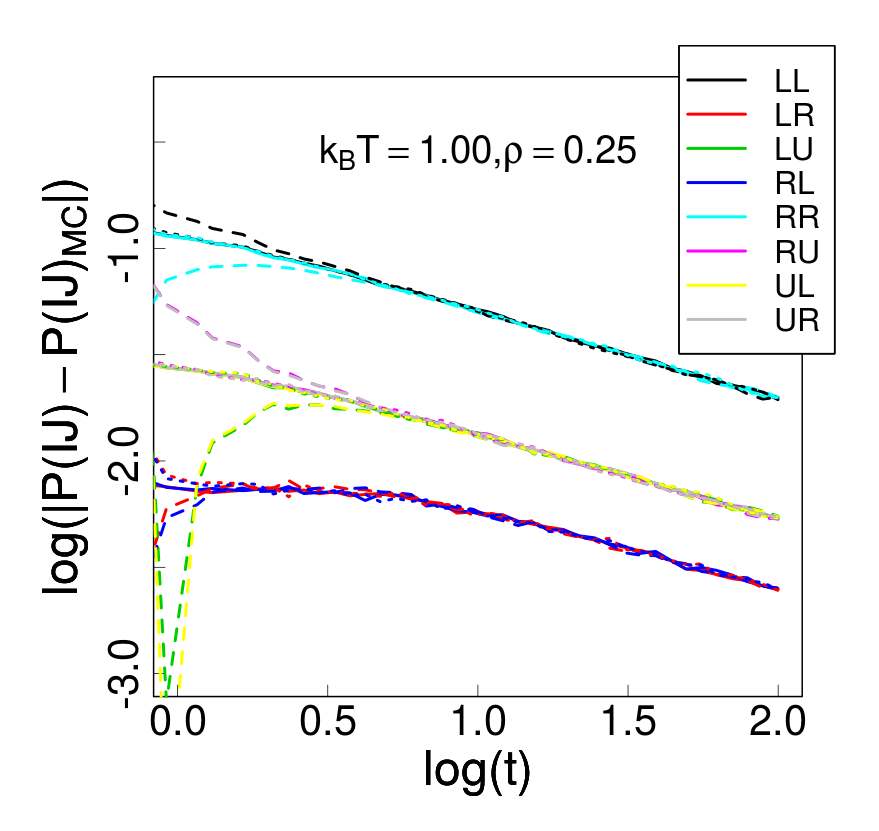
\includegraphics[width=\textwidth]{Images/relax_1_25.png}
	\captionsetup{justification=centering, width=0.9\columnwidth}
\end{subfigure}
\begin{subfigure}[t]{0.45\textwidth}
	\centering
	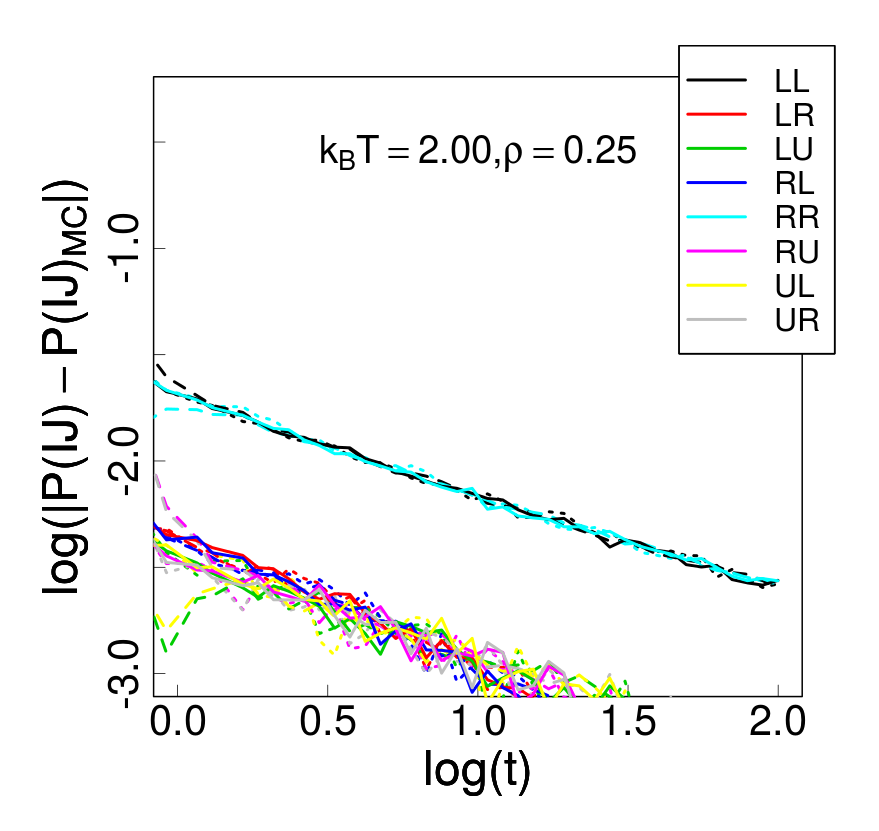
\includegraphics[width=\textwidth]{Images/relax_2_25.png}
	\captionsetup{justification=centering, width=0.9\columnwidth}
\end{subfigure}
\centering
\begin{subfigure}[t]{0.45\textwidth}
	\centering
	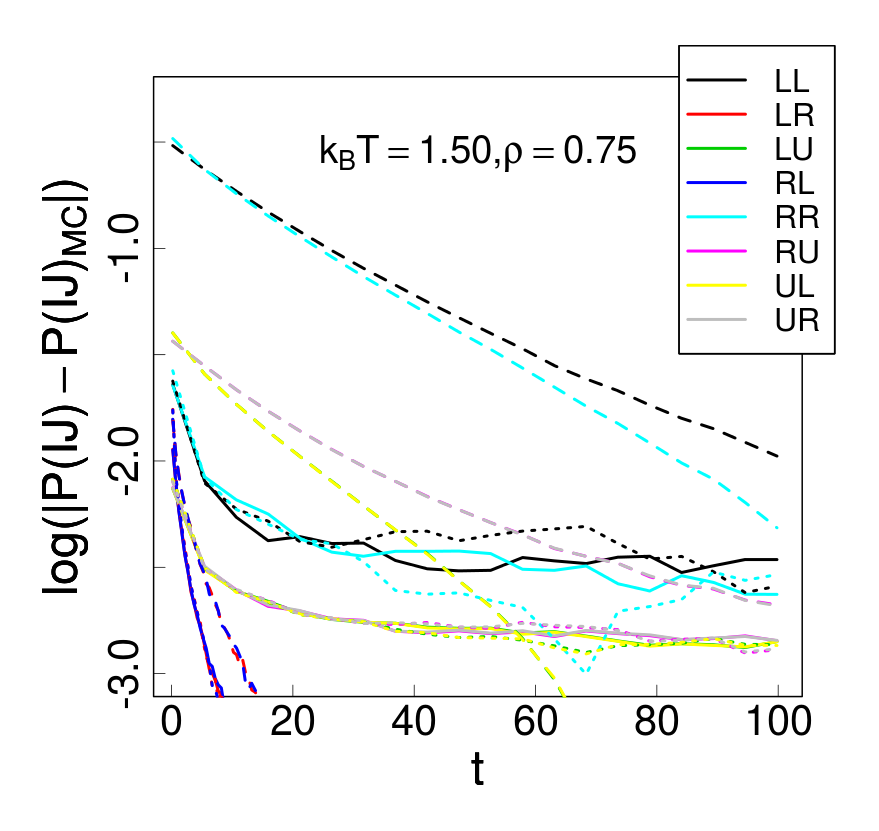
\includegraphics[width=\textwidth]{Images/relax_15_75.png}
	\captionsetup{justification=centering, width=0.9\columnwidth}
\end{subfigure}
\begin{subfigure}[t]{0.45\textwidth}
	\centering
	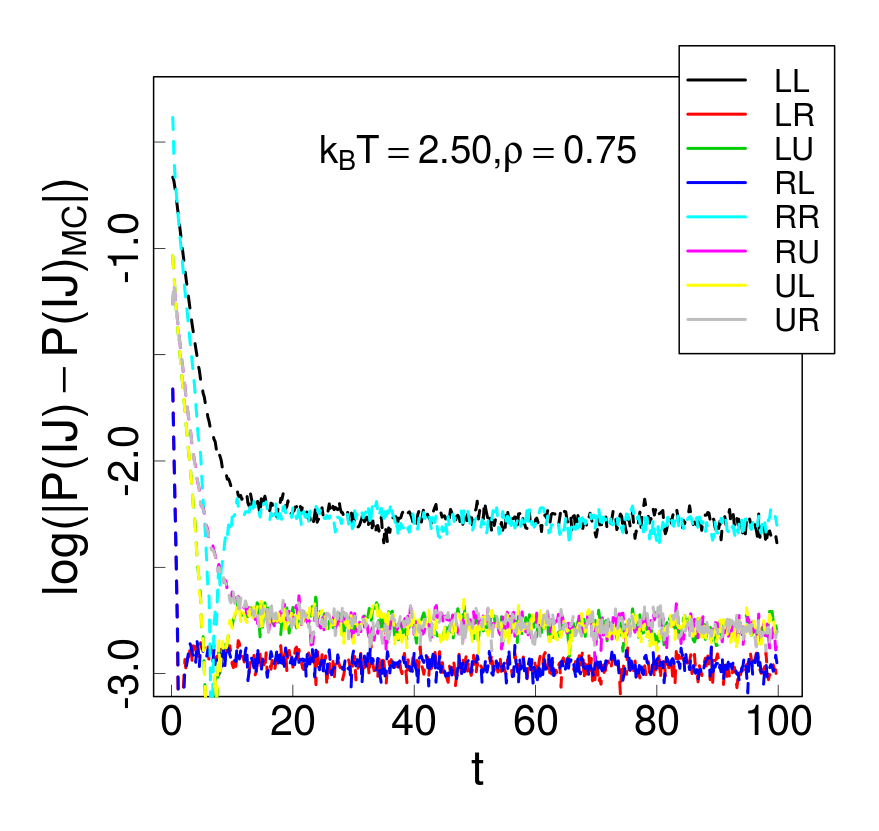
\includegraphics[width=\textwidth]{Images/relax_25_75.png}
	\captionsetup{justification=centering, width=0.9\columnwidth}
\end{subfigure}
\captionsetup{justification=centering, width=0.9\columnwidth}
\caption{Probabilities of having different pairs orientations as function of simulation time for different $k_BT$ and $\rho$. Solid lines indicates random initial configuration, small dashes --- co-aligned, and long dashed --- counter-aligned. The simulations are performed for $N = 6400$ particles and the results are averaged over $500$ samples}
\label{fig:short_time_probs_different_density}
\end{figure}

\textcolor{red}{Hello Nuno! Hope you do not want to fire me right away after you read this. If not, I want to do more careful comparison of probability relaxations for small density (if they are with the same slope or not), and maybe longer simulations for both MD and MC cases, because for high density it looks really strange. Even if you want to fire me (which, I hope you don't), I would like to show you the results for all densities and $k_BT$s I have on Monday, because for me they just do not make sense as a whole}